\section{Fusion}
Kärnreaktorer har ni säkert hört talas om. Oftast funkar dessa genom att klyva atomkärnor, det vill säga utföra \emph{fission}. Stjärnor gör något liknande, men de sätter ihop atomkärnor i stället för att klyva isär dem. Detta heter \emph{fusion}. Det krävs väldigt höga tryck och temperaturer för att möjliggöra fusion, men i vissa fall ger processen mer energi ut än som sattes in, vilket är det som bland annat möjliggör stjärnor.

Både fission och fusion fungerar eftersom olika atomer har olika \emph{bindningsenergi}. Det finns nämligen en viss energi som krävs för att se till att nukleonerna i atomkärnan inte flyger iväg. Bindningsenergin är också förvånansvärt stor. Vi har svårt att mäta den direkt, men man kan använda Einsteins materia-energiekvivalens:
\begin{equation}
    E = mc^2
    \label{eq:emc2}
\end{equation}
i stället.

Ekvivalensen säger att den totala energin lagrat i ett visst föremål är lika med dess massa gånger ljusets hastighet i kvadrat. Med hjälp av detta kan vi observera skillnaden i energi mellan samma molekyl i olika tillstånd. Till exempel kommer energin för 2 lösa protoner (\ce{2p+}) och 2 lösa neutroner (\ce{2n}) vara större än dessa sammansatta för att bilda en \ce{^2_4He^2+} kärna som ni kan se i \cref{tab:helium-energy}. En elektrons massa är försumbart liten i detta sammanhang, och deltar därför inte i beräkningarna.

Denna relation kan även tillämpas för skillnaden mellan två fria atomkärnor och en större atomkärna bildad genom att \emph{fusionera} --- sätta samman till ett --- de två kärnorna. För lika par av grundämnen gäller det att deras fusionsprodukt alltid har lite lägre energi än de skiljda upp till järnatomen. Efter järn har fusionsprodukten av ett likt par grundämnen lite mer energi fusionerat än separat.

Detta innebär i slutändan att fusionsreaktioner av lika atompar ger ett energiöverskott för grundämnen upp till järn. Detta överskott blir till värme. Den extra energin är ganska liten jämfört med energin som krävs för att trycka ihop atomkärnorna men är inte försumbar i stora skalor med många atomer samtidigt.

\begin{table}[b]
    \def\arraystretch{1.5}
    \centering
    \caption{Energin för heliums beståndsdelar och dess kärna.}
    \label{tab:helium-energy}
    \begin{tabular}{c|c|c}
        \textbf{Sak} & \textbf{Massa (kg)} & \textbf{Energi (J)} \\\toprule
        \ce{2p+ + 2n} & \qty{6.696e-27}{kg} & \qty{6.018e-10}{J}\\
        \ce{^2_4He^2+} & \qty{6.646e-27}{kg} & \qty{5.974e-10}{J} \\\bottomrule
        \textbf{Differens} & \qty{5e-30}{kg} & \qty{4.4e-12}{J}

    \end{tabular}
\end{table}

\section{Stjärnornas anatomi}
En stjärna är i grund och botten en boll av gas. Först och främst består dem av väte (\ce{H}) och helium (\ce{He}). De innehåller dock ämnen hela vägen upp till järn (\ce{Fe}) i periodiska systemet (se \vref{fig:periodic-table} för ett periodiskt system).

Deras inre struktur kan liknas till en lök. Ju större, och äldre, en stjärna är desto fler lager har den. Man kan betrakta stjärnan som en fusionerande kärna och ett icke-fusionerade yttre lager samt en atmosfär. ''Kärnan'' är ett missvisande begrepp här, eftersom det som faktiskt kallas \emph{kärna} är endast det innersta lagret. Dock finns det i äldre stjärnor fusionerande lager runt kärnan. Atmosfären är distinkt från det icke-fusionerande lagret eftersom den är genomskinlig för ljus, till skillnad från de inre lagren. Ett diagram för en äldre stjärna av stor massa finns i \cref{fig:star-anatomy}.
\begin{figure}[h!]
    \centering
    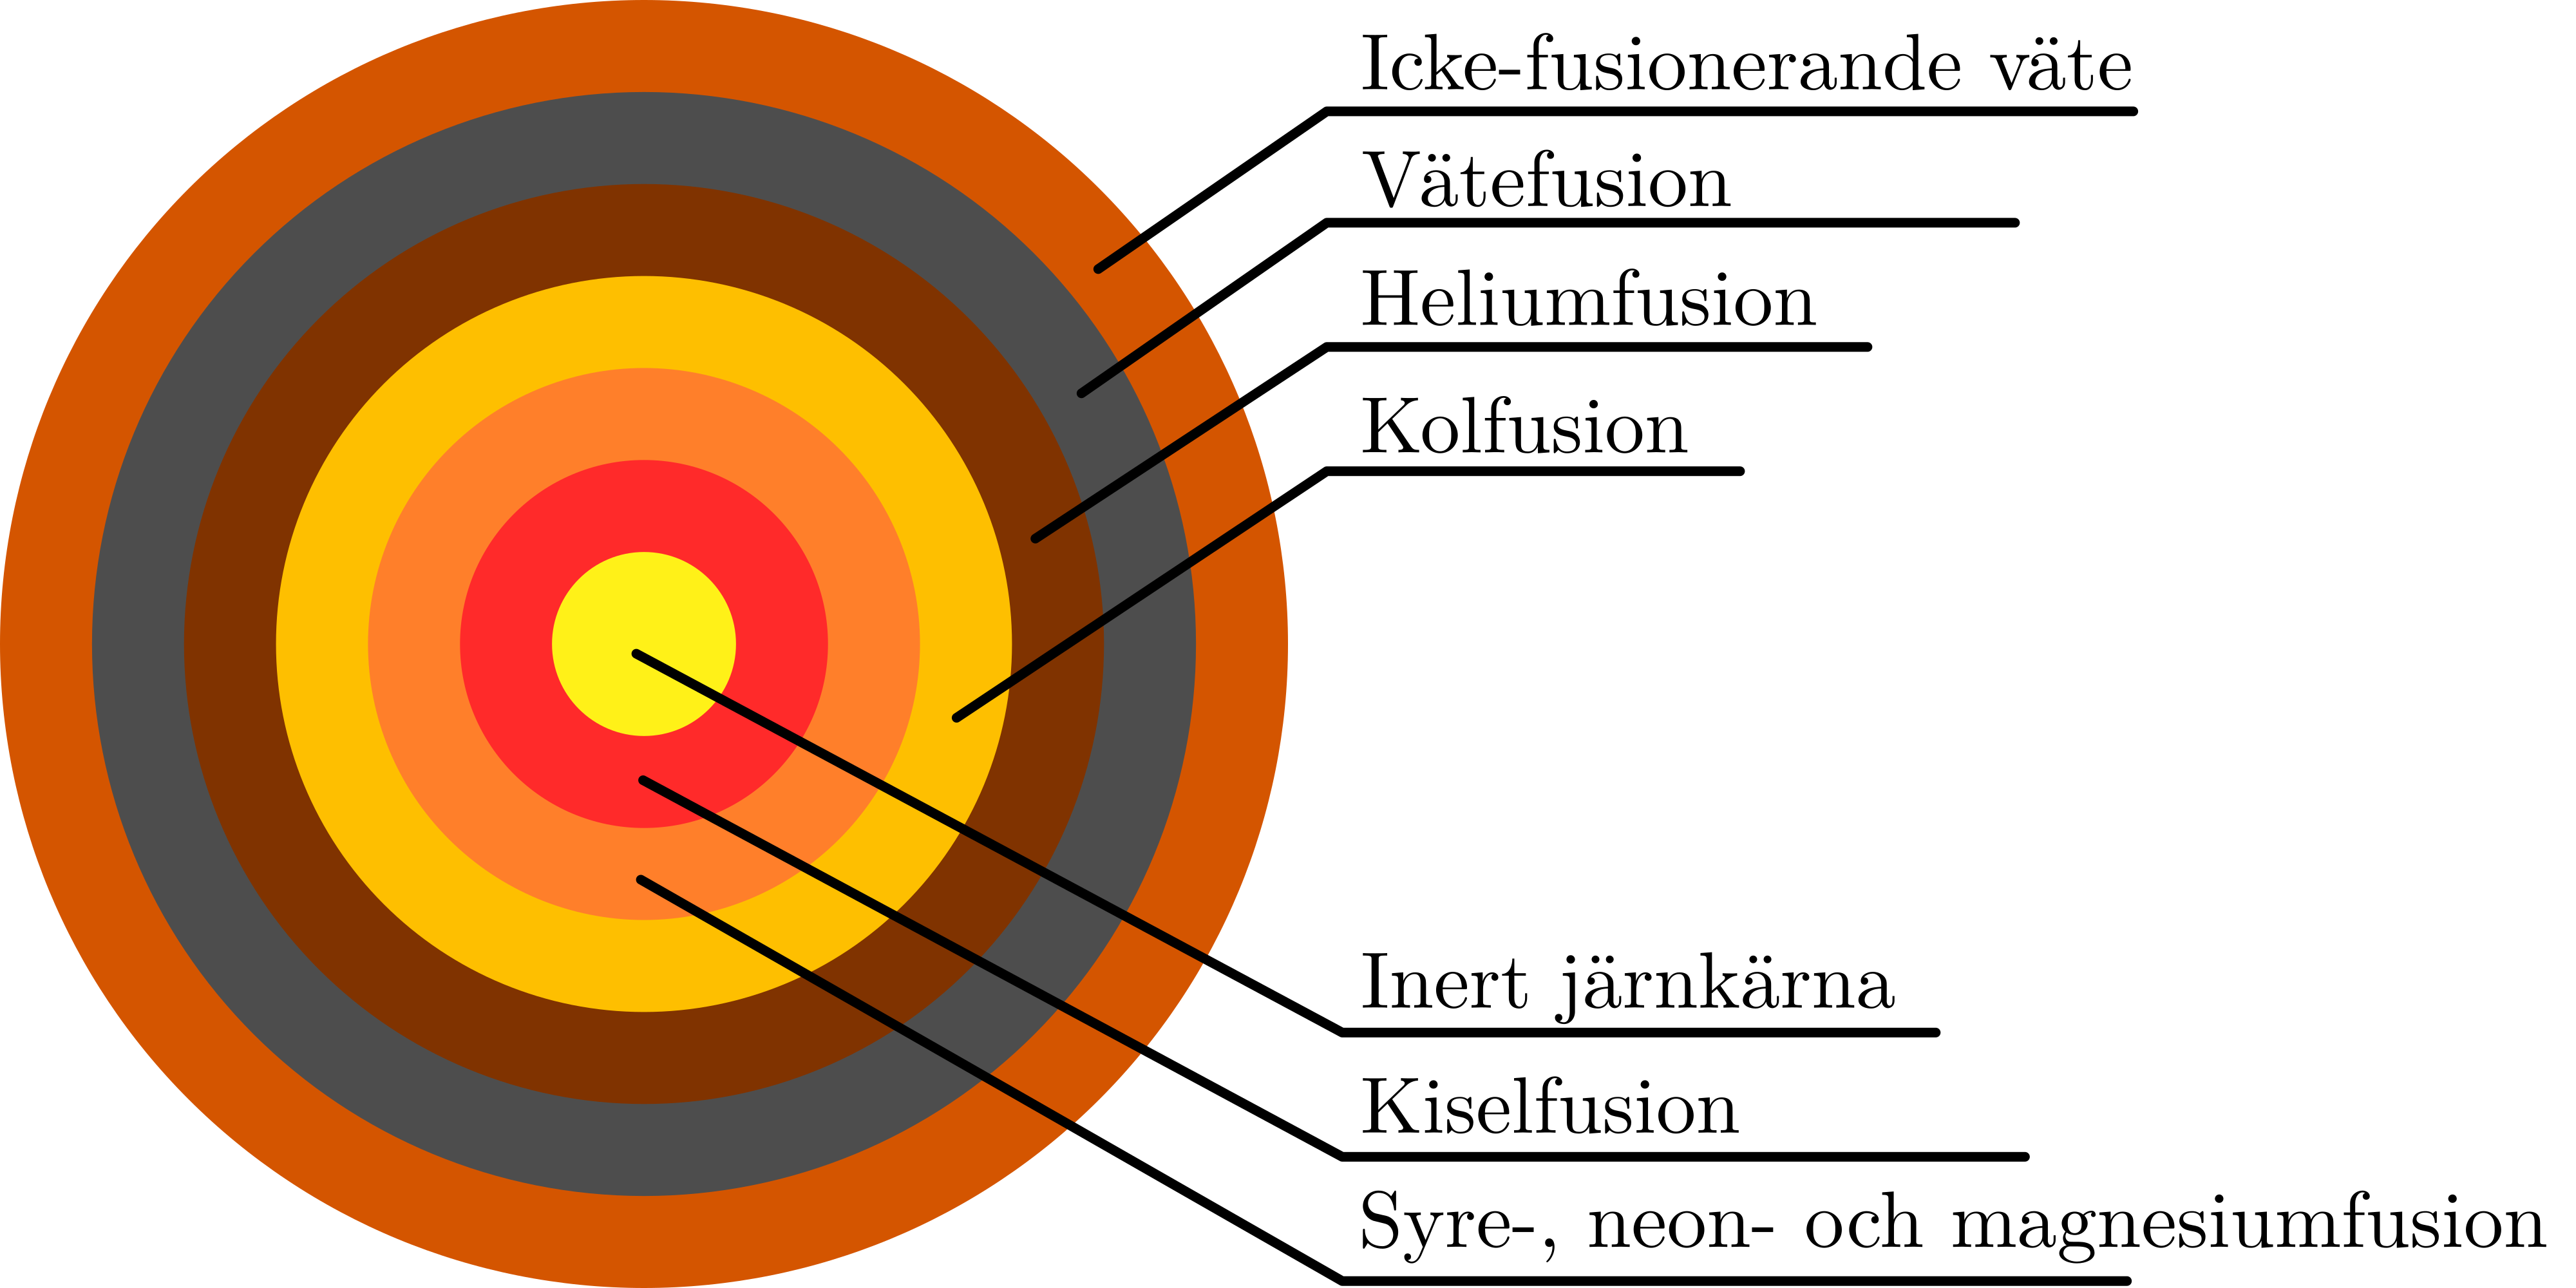
\includegraphics[width=0.8\textwidth]{img/star.png}
    \caption{En massiv, gammal stjärnas inre struktur.}
    \label{fig:star-anatomy}
\end{figure}

\section{Stjärnors livscykel}
En stjärnas liv består i huvudsak av tre steg: (i) födelse, (ii) huvudsekvens och (iii) väg till döden. Alla stjärnor föds och lever på huvudsekvensen, dock dör olika stjärnor på olika sätt.

Stjärnor föds genom att gas från rymden samlas tack vare gravitation på en punkt. När denna gasklump blir massiv nog, det vill säga cirka \qty{0.08}{\Mo}, kommer vätefusion att inledas. Då börjar stjärnan dess existens på den så kallade \emph{huvudsekvensen}. Under denna tid samlas helium som lagras i kärnan. Vad som händer sen beror på typen av stjärna.

\subsection{Små stjärnor}
Små stjärnor mindre än ca \qty{0.5}{\Mo} kommer aldrig att kunna fusionerna helium då de saknar massan för att skapa tillräckligt med tryck. De kommer stanna på huvudsekvensen länge, upp till flera biljarder ($10^{12}$) år. När de har bränt upp allt väte kommer de att kollapsa till en vit dvärg.

\subsection{Medelstora stjärnor}
Stjärnor mellan \qtyrange{0.5}{2.25}{\Mo} har nog med massa för att fusionera helium. De kommer först att ansamla helium i kärnan utan att fusionera det. Till slut kommer heliumet blir så mycket att det tvingar ut vätet och stjärnan får en icke-fusionerande kärna med ett lager av vätefusion runt som tillför nytt helium hela tiden. Detta orsakar att stjärnan växer till att bli mycket större och blåsa iväg en stor andel av sin yttre massa. Därefter kallas stjärnan för en \emph{röd jätte}. Solen kommer till slut att bli en röd jätten, och då kommer den bli \num{250} ggr. större och tappa \qty{30}{\percent} av sin massa.

Till slut blir kärnan stor nog för att fusionerna helium och då kommer denna fusion plötsligt att börja. Detta heter \emph{helium flash}. Då krymper också stjärnan och blir mycket varmare på ytan.

När nog med kol bildats från helium kommer även heliumet flytta ut till ett skikt runt den varma, men icke-fusionerande kolkärnan. Kolet går dock inte att fusionera längre vid denna massa, så stjärnan kommer över tid att förbruka sitt bränsle.

\subsection{Stora stjärnor}
För stjärnor \qtyrange{2.25}{4}{\Mo} händer samma sak som ovan, men heliumfusion börjar lite smått redan innan skikten bildas och stjärnan går över till att vara en jätte.

\subsection{De största stjärnorna}
Stjärnor \qty{>9}{\Mo} blir först blåa jättar och sedan röda jättar. Om massan är \qty{>40}{\Mo} kommer stjärnan aldrig blir röd jätte eftersom den tappar för mycket massa. Om större stjärnor uppfyller massan för att fusionera element tyngre än helium kommer de utvecklas längre än de mindre stjärnorna. Exempelvis kommer kolkärnan att fusioneras efter ett tag, med helium och väteskikt runt. Sedan kommer det att bli tyngre och tyngre element i mitten när temperaturen successivt ökar. Vid järn upphör energipositiv fusion och stjärnan kollapsar under sin egna vikt.

\subsection{Kollaps}
När fusion upphör kommer stjärnan att kollapsa. För små stjärnor blir det som sagt direkt en vi dvärg. Detta gäller för massor \qty{<1.4}{\Mo}. För stjärnor med \qtyrange{1.4}{4}{\Mo} kommer det bli en supernova, en stor explosion, sedan en neutronstjärna kvar. För större stjärnor blir det i stället ett svart hål då neutronstjärnan inte klarar att hålla upp sig själv under dess egna vikt.


\section{Stjärnors ljus}
Stjärnor lyser eftersom de är varma. Alla föremål som har en temperatur större än absoluta nollpunkten avger ljus av något slag ($\qty{0}{K} = \qty{-273.15}{\degreeCelsius}$). Till och med du som läser detta lyser! (dock osynligt.) Denna strålning heter svartkroppsstrålning och avger lite av alla våglängder av ljus. Den heter ''svartkropp'' eftersom det är strålningen en perfekt, svart kropp skulle avge vid en given temperatur. En perfekt, svart kropp här innebär ett ogenomskinligt föremål som inte reflekterar något ljus.
